\chapter{CPLEX}

Per poter utilizzare gli algoritmi di risoluzione forniti da CPLEX è necessario costruire il modello del problema legato all'istanza sopra descritta.\\
CPLEX possiede due meccanismi di acquisizione del modello:

\begin{itemize}
\item{modalità interattiva: in cui il modello viene letto da un file precedentemente generato (\textit{model.lp})}
\item{definendo il modello attraverso le API del linguaggio C (o del linguaggio utilizzato per la scrittura del programma)}
\end{itemize}

Per memorizzare tale modello CPLEX utilizza due strutture dati:

\begin{itemize}
\item{ENV (enviroment): contiene i parametri necessari all'esecuzione}
\item{LP: contiene i dati degli elementi del modello}
\end{itemize}

%inserire immagine

Ad ogni ENV è possibile associare più LP, ma nel nostro caso ne sarà sufficiente uno solo.\\

Come prima cosa, per poter costruire il modello da analizzare, è necessario creare un puntatore alle due strutture dati necessarie a CPLEX.\\

\lstinputlisting[caption={\footnotesize{modelTSP.txt}}, style=code, firstnumber=1, firstline=27, lastline=29, label=tsp_model, language=c]{Source/modelTSP.txt}

La funzione alla riga 2 alloca la memoria necessaria e riempie la struttura con valori di default. Nel caso in cui non termini con successo memorizza un codice d'errore in \textit{\&errore}. La funziona invocata nella riga successiva, invece, associa la struttura LP all'enviroment che gli viene fornito. "TSP" sarà il nome del modello creato.\\
Al termine di queste operazioni il modello, riempirlo è stata costruita la seguente funzione:\\

\begin{lstlisting}[linewidth=250pt, basicstyle=\footnotesize\sffamily,]     
build_model(&instanza_problema, env, lp);
\end{lstlisting}

Viene aggiunta al modello una colonna alla volta con i costi dei vari archi, sfruttando \\

\begin{lstlisting}[linewidth=350pt, basicstyle=\footnotesize\sffamily,]     
CPXnewcols(env, lp, num_colonne, vettore_costi,
 vettore_lower_bound, vettore_upper_bound, dato_binario, 
 stringhe_nomi);
\end{lstlisting}

Questa funzione aggiunge \textit{num\_colonne} colonne con una sola invocazione, per far si che ne aggiunga una sola è necessario passargli l'indirizzo di \textit{vettore\_costi, vettore\_lower\_bound, vettore\_upper\_bound, dato\_binario, stringhe\_nomi} affinché li veda come array da un elemento e non come variabili.

Per poter inserire il primo vincolo del problema\\

$$
\underset{e\in \delta(v)}\sum{\;x_e} = 2\;\;\;\;\;\;\;\;\;\;\;\;\;\;\;\;\;\;\forall\;v\in V \\\\
$$
\\
viene sfruttata la funzione \\

\begin{lstlisting}[linewidth=350pt, basicstyle=\footnotesize\sffamily,]     
 CPXnewrows(env, lp, numero_righe, vettore_termini_noti,
  vettore_tipo_vincoli, NULL, stringhe_nomi);
\end{lstlisting}

Anche in questo caso è necessario seguire le stesse accortezze dell'analoga sopra descritta poiché inserisce \textit{numero\_righe} alla volta.\\
In questo modo si viene a creare una matrice in cui è presente il valore 1 se il nodo in questione appartiene al ramo nella colonna corrispondente, 0 altrimenti.\\
Per convenzione è stato deciso di indicare tutti i rami $(i,j)$, con $i\neq j$, rispettando la proprietà $i<j$. Per tener conto di questo particolarità è necessario fare particolare attenzione nell'inserimento delle righe.\\

\begin{figure}[h!] 
\begin{center} 
  % Requires \usepackage{graphicx} 
  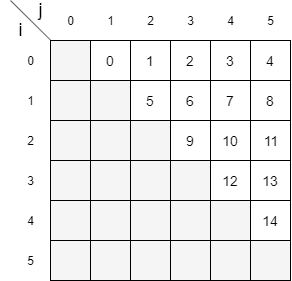
\includegraphics[width=14cm]{Images/indices_matrix}\\ 
  \caption{} 
\end{center} 
\end{figure}


%inserire immagine



